%<dscrpt>Nombre de sphères tangentes extérieurement à une sphère donnée.</dscrpt>
\begin{figure}[h!t]
 \centering
 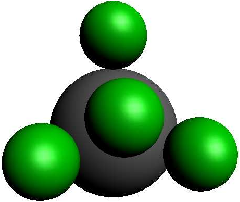
\includegraphics{./Esphertan_1.pdf}
 \caption{Une $\frac{1}{2}$-configuration de $4$ sphères disjointes.}
 \label{fig:Esphertan_1}
\end{figure}
Dans un espace euclidien de dimension $3$, pour un réel $r>0$, une $r$-configuration est un ensemble de sphères de rayon $r$ et tangentes extérieurement à la sphère unité. L'intersection de deux d'entre elle doit contenir au plus un point. Elles peuvent donc être disjointes ou tangentes mais pas se couper. Pour une $r$-configuration de $m$ sphères, on notera $S_1,\cdots,S_m$ ces sphères et $A_1,\cdots,A_m$ leurs centres.\newline
L'objet de ce problème\footnote{d'après \'Ecole de l'air 1993} est de donner des propriétés du plus grand des cardinaux des $r$-configurations pour un $r$ donné. Il est noté $n(r)$.
\begin{enumerate}
 \item Montrer que $r\rightarrow n(r)$ est une fonction décroissante.
 \item Montrer que $n(r)\geq 2$ pour tout $r>0$.
 \item Pour une $r$-configuration de $m$ sphères et $i\neq j$ entre $1$ et $n$, en considérant $\Vert \overrightarrow{A_iA_j}\Vert^2$, montrer que le cosinus de l'écart angulaire entre $\overrightarrow{OA_i}$ et $\overrightarrow{OA_j}$ est inférieur ou égal à
\begin{displaymath}
 1-2\left( \frac{r}{1+r}\right)^2
\end{displaymath}
\item 
\begin{enumerate}
 \item En développant $\left\Vert \sum_{i=1}^3 \overrightarrow{OA_i}\right \Vert^2$, montrer que $r> 2\sqrt{3}+3$ entraine $n(r)=2$.
 \item En développant $\left\Vert \sum_{i=1}^4 \overrightarrow{OA_i}\right \Vert^2$, montrer que $r>\sqrt{6}+2$ entraine $n(r)\leq 3$.
\end{enumerate}
\begin{figure}[h!t]
 \centering
 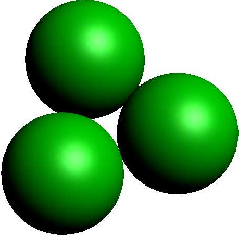
\includegraphics{./Esphertan_2.pdf}
 \caption{Triangle équilatéral.}
 \label{fig:Esphertan_2}
\end{figure}
\item En considérant des polyèdres réguliers et des homothéties, on forme des configurations particulières qui conduisent à de nouvelles inégalités.
\begin{enumerate}
 \item On considère un triangle équilatéral inscrit dans un cercle de rayon $R$. Quelle est la distance entre deux sommets? Montrer que $r\leq 2\sqrt{3}+3$ entraine $n(r)\geq 3$.
\begin{figure}[h!t]
 \centering
 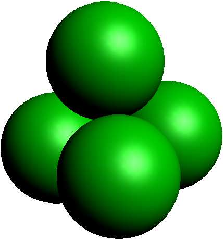
\includegraphics{./Esphertan_3.pdf}
 \caption{Tétraèdre régulier.}
 \label{fig:Esphertan_3}
\end{figure}

 \item Un repère orthonormal étant fixé, on considère un tétraèdre dont les sommets sont les quatre points respectivement de coordonnées
\begin{displaymath}
 (1,1,1),\hspace{0.5cm}(1,-1,-1),\hspace{0.5cm}(-1,1,-1),\hspace{0.5cm}(-1,-1,1),\hspace{0.5cm}
\end{displaymath}
Quelle est la distance entre deux sommets?\newline Montrer que $r\leq \sqrt{6}+2$ entraine $n(r)\geq 4$.

\item On utilise cette fois les sommets, les milieux des arêtes et les milieux des faces d'un cube.\newline
Que conclure sur $n(r)$ lorsque $r$ est inférieur ou égal à $\sqrt{2}+1$, $\frac{\sqrt{3}+1}{2}$, 1 ?
\end{enumerate}
\begin{figure}[h!t]
 \centering
 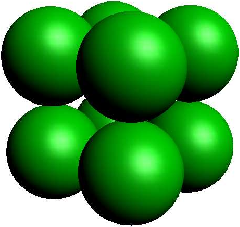
\includegraphics{./Esphertan_4.pdf}
 \caption{Sommets d'un cube.}
 \label{fig:Esphertan_4}
\end{figure}
\begin{figure}[h!t]
 \centering
 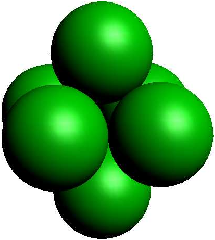
\includegraphics{./Esphertan_5.pdf}
 \caption{Milieux des faces d'un cube.}
 \label{fig:Esphertan_5}
\end{figure}
\begin{figure}[h!t]
 \centering
 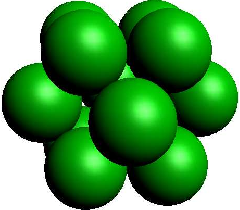
\includegraphics{./Esphertan_6.pdf}
 \caption{Milieux des arêtes d'un cube.}
 \label{fig:Esphertan_6}
\end{figure}

\item Pour $s\in]-1,1[$, on considère la région de la sphère unité formée par les points $m$ tels que $x(m)\geq s$. On admet que l'aire de cette région est $2\pi(1-s)$.
\begin{enumerate}
 \item Pour une sphère $S_i$ de rayon $r$ et tangente extérieurement à la sphère unité, on considère l'ensemble $\Sigma_i$ des points d'intersection de la sphère unité avec les demi-droites $(Om)$ pour $m\in S_i$. Montrer que l'aire de $\Sigma_i$ est
\begin{displaymath}
 2\pi\left( 1- \frac{\sqrt{1+2r}}{1+r}\right) 
\end{displaymath}
 \item Montrer que
\begin{displaymath}
 n(r)\leq \frac{2(1+r)(1+r+\sqrt{1+2r})}{r^2}=a(r)
\end{displaymath}
\end{enumerate}
\item On rappelle que le volume d'une boule de rayon $R$ est $\frac{4}{3}\pi R^3$. En considérant des volumes, préciser une fonction $v(r)$ telle que $n(r)\leq v(r)$.
\item Former, pour $r$ au voisinage de $0$, des développements de $a(r)$ et de $v(r)$. Quelle est la meilleure des deux majorations ?
\end{enumerate}
 